\documentclass[12pt,fleqn]{article}\usepackage{../common}
\begin{document}
Ders 1

Konumuz Kismi Turevsel Denklemler (partial differential equtions -PDE-). Bu
dersin on gerekliliklerinden en onemlisi normal diferansiyel denklemlerdir
(ordinary differential equtions -ODE-), cunku pek cok PDE'yi cozmenin
teknigi onlari bir ODE sistemine indirgemekten geciyor. Yani PDE cozmek
icin ODE cozme tekniklerini de bilmek gerekiyor. Bir diger gerekli bilgi
Lineer Cebir dersi.

Bu dersin ana amaci, bir muhendislik dersi olarak, denklem cozmek, ve pek
cok denklemin cikis noktasi fiziksel problemler. Mesela sicaklik yayilmasi
(heat diffusion), dalga hareketi (wave motion), titresen hucre zari
(vibrating membrane) gibi. Fakat PDE kavrami finansta bile ortaya cikabilen
bir kavram, mesela Black-Sholes denklemlerinde oldugu gibi. 

Yani dersimiz cok teori odakli olmayacak, bazi ispatlardan bahsedecegiz,
ama onun haricinde teori uzerinde fazla durmayacagiz. 

PDE nedir? Ilk once ODE tanimindan baslayalim. 

\[ y = y(x) \]

\[ \frac{dy}{dx} = y \]

Baslangic sartlari 

\[ y(0) = y_0 \]

Cozum 

\[ y = y_0e^x \]

Bu bir ODE cunku sadece bir tane bagimsiz degisken var ($x$), ve bir tane
bagimli degisken var ($y$). 

PDE ise icinde kismi turevleri, ve bir veya {\em birden fazla} bagimsiz
degiskeni barindiran bir denklemdir.

Eger gunes etrafindaki yorungeleri temsil etmek istiyorsaniz gezegenleri
boyutsuz parcaciklar gibi kabul ederek ODE'ler ile temsil etmek yeterli
olabilir, ama diger problemlerde daha fazla bagimsiz degisken gerekecegi
icin ODE yetmez, mesela zaman, cismin 3D uzaydaki boyutlari gibi.

Mesela bir PDE

\[ u = u(x,y) \]

Cogunlukla problem taniminin ilk basinda fonksiyonel iliskiyi hemen
gostermek iyi olur, mesela ustte bagimsiz degiskenler $x,y$, ve $u$ bu iki
degiskene bagimli. Devam edelim PDE soyle olsun

\[ \frac{\partial^3 u}{\partial x^3} + 
cos(y)\frac{\partial u}{\partial y} + 3 = 0
\]

Bir PDE problemine cogunlukla ek olarak sinir kosullari (boundary condition
-BC-) ve baslangic kosullari (initial conditions -IC-) eklemek de gerekir. 

Kismi Turev nedir? 

\[ u = u(x_1, x_2,...,x_n) \]

\[ 
\frac{\partial u}{\partial x_i} = 
\lim_{\Delta x_i \to 0} 
\frac{
u(x_1,..,x_i+\Delta x_i,x_{i+1},...,x_n) - u(x_1,..,x_i,x_{i+1},...,x_n)}
{\Delta x_i}  \]

Yani bir fonksiyonun kismi turevini almak istedigimiz degisken haricinde
tum diger degiskenlerinin sabit tutuldugu bir durum. 

Ornek

\[ u = x_1^2 + x_1sin(x_2) \]

\[ 
\frac{\partial u}{\partial x_1} = 2x_1 + sin(x_2)
 \]

\[ 
\frac{\partial u}{\partial x_2} = x_1 cos(x_2)
 \]

Notasyon

Cogunlukla kismi turevler 3 farkli sekilde gosteriliyor. 

\[ \frac{\partial u}{\partial x} \equiv u_x \equiv \partial_x u \]

Ustte soldaki tanimi gorduk, bazen ortadaki de tercih edilebiliyor, ya da
bazen en sagdaki. 

PDE Derecesi

Bir PDE'nin derecesi, o denklemdeki kismi turevlerin en yuksek dereceli
olanin derecesi neyse o'dur.

Mesela

\[ u_{xxx} + u_y = 5 \]

derecesi 3. Ayni zamanda bu lineer ve homojen olmayan (inhomogeneous) bir
PDE. Bu son iki kavrami birazdan tanimlayacagim. 

Ornek 

\[ (u_{xx})^2 + u_xu_y = u \]

Bu 2. derece. Bu bazi insanlarin kafasini karistiriyor, cunku $u_{xx}$'in
karesi var. Bu ayni zamanda homojen, ve gayri lineer. Bu dersteki cogu PDE
lineer olacak. 

Lineer ve gayri lineerlikten bahsetmisken, sunu ekleyelim. 

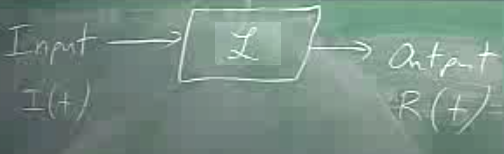
\includegraphics[height=3cm]{1_5.png}

Simdi diyelim ki bir girdi (input) fonksiyonu $I(t)$ bir isleme giriyor
($L$ operatoru) ve cikti (output) olarak $R(t)$ cikiyor. Yani sistem

\[ R = \mathcal{L} \ I \]

Bir lineer sistemde eger girdiyi iki ile carparsaniz, cikti da iki katina
cikar. O zaman kurallar

\begin{enumerate}

   \item $\mathcal{L}(\alpha I) = \alpha \ \mathcal{L}(I)$, ki $\alpha$ bir sabit.

   \item $\mathcal{L}(I_1 + I_2) = \mathcal{L}(I_1) + \mathcal{L}(I_2)$, ki buna ust uste eklenebilme
     (superposition) prensibi deniyor. Bu prensibi bu dersteki cogu PDE'yi
     cozmek icin kullanacagiz. Bir lineer sistem varsa cogu zaman arka
     planda bir yerlerde ust uste eklenebilme prensibi geziniyordur. 

\end{enumerate}

Diyelim ki PDE'nizi soyle yazdiniz

\[\mathcal{L}u = f(\vec{x}) \]

Burada $u$ bagimli degisken, $\vec{x}$ bir vektor, $\vec{x} \in \mathbb{R} ^n$, ve
bu vektorun icinde birden fazla degisken var, bu degiskenlerin hepsi
bagimsiz.

\[ 
\vec{x} = 
\left(\begin{array}{r}
x_1,\\
.. \\
x_n
\end{array}\right)
 \]

Bu denkleme benzer bir diger denklem lineer cebirdeki $A\vec{x} = \vec{b}$
denklemidir.  PDE sisteminde de cevabini aradigimiz, lineer cebir
sisteminde ``$A$ ile carpilip $b$ sonucunu verecek $\vec{x}$ hangisidir?''
sorusuna benzer bir sekilde ``$\mathcal{L}$ operatoru uygulanip $f(\vec{x})$
sonucunu verecek $u$ hangisidir?'' sorusudur.

Bu analojiden devam etmek gerekirse, belli bir noktada $u$'nun icinde
oldugu ``fonksiyon uzayi'' hakkinda dusunmemiz gerekebilir, $\vec{x}$'in
icinde oldugu $\mathbb{R}^n$ uzayi gibi. Lineer cebir durumunda operatorun
ozelliklerine bakilir, mesela `` $b$'nin icinde oldugu ve $A$ operatoru
uygulanip hic sonuc alinamayacak uzayin belli kisimlari var
midir?'' gibi sorularla ugrasilabilir, bunlar $A$'nin ``ulasamadigi
yerlerdir'' vs. PDE'deki $\mathcal{L}$ operatoru icin de benzer sorular sorulabilir. 

Yani lineer cebirle pek cok kavram PDE dunyasina benziyor, orada vektor
uzayi var, burada fonksiyon uzayi var. Yani bir analoji olarak bu
benzerligi aklimizda tutmamiz faydali. 

Bir operator su sekilde de olabilir

\[ \mathcal{L} = \mathcal{L} \bigg(
\frac{\partial }{\partial x_1}, \frac{\partial }{\partial x_2},..,
u,..
\bigg)
 \]

Yani operator kismi turevlere ve hatta $u$'nun kendisine de bagimli
olabilir. 

Eger elimizde gayri lineer bir PDE var ise, basimiz dertte demektir. Boyle
bir sistemi cozmek icin cogunlukla sayisal cozumlere basvurmak
gerekir. Eger lineer ise cozumde bayagi ilerlemek mumkundur. 

Lineerlik

Bir operator ve onun tanimladigi bir ust uste eklenebilme durumu dusunelim

\[ \mathcal{L} = \mathcal{L}(\alpha_1 u_1 + \alpha_2 u_2) = 
\alpha_1 \mathcal{L}u_1 + \alpha_2 \mathcal{L}u_2 \]

ki $\alpha_1,\alpha_2$ birer tekil sayidir (scalar), ya reel, ya da kompleks. 

Ornek

Birazdan bakacagimiz denklem dalga denklemi. Orada

\[ u_{tt} - c^2u_x = 0 \]

Bu denklemi

\[ \mathcal{L}u = 0 \]

seklinde yazabiliriz ki $\mathcal{L}$ soyle tanimli olacaktir

\[ \mathcal{L} = \frac{\partial^2}{\partial t^2} - 
c^2 \frac{\partial ^2}{\partial x^2 = 0}\]

$c$ bir sabittir. 

Simdi diyelim ki su denklemi cozmemiz lazim

\[\mathcal{L} u = f \]

ki

\[ \mathcal{L}: V \to V \]

Yani, $\mathcal{L}$ bir vektor uzayini bir digerine eslemekte (map), ve yine diyelim
ki bu uzaylar birer Hilbert Uzayi (bunun anlamina simdi bilmemiz
gerekmiyor, ileride bu konuya donecegiz, bu kelimeyi soyle bir ortaya atmak
istedim). 

Yani sordugumuz Hilbert Uzayi $V$'de bir $f$'e esleyecek bir $u$ fonksiyonu
olup olmadigi. Bu arada tipik bir Hilbert Uzayi mesela kare alip bir sinir
bolgesinde (boundary domain) entegre edince elde edilen sonlu (finite) bir
sonuclarin olusturdugu uzay. Yani ``derli toplu'' fonksiyonlar bir anlamda,
absurt sonuclar vermeyen turden, sonsuzluga dogru patlayip giden turden
olanlari degil. 

Faraziyeye devam edelim, diyelim ki $V$ icinde bir baz (basis) var. Baz
nedir? Lineer cebirden hatirlayalim, mesela uc boyutlu Oklidsel (Euclidian)
uzayi $\mathbb{R}^3$. 

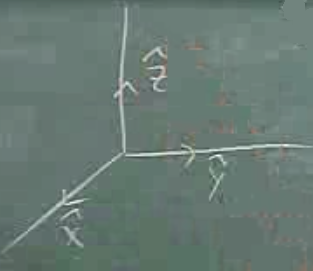
\includegraphics[height=4cm]{1_6.png}


\[ 
\vec{x} = 
\left[\begin{array}{r}
1 \\ 0 \\ 0
\end{array}\right]
 \]

\[ 
\vec{y} = 
\left[\begin{array}{r}
0 \\ 1 \\ 0
\end{array}\right]
 \]

\[ 
\vec{z} = 
\left[\begin{array}{r}
0 \\ 0 \\ 1
\end{array}\right]
 \]

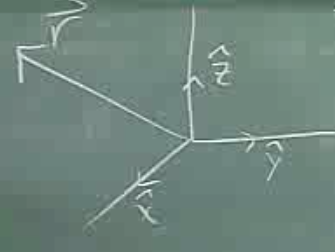
\includegraphics[height=4cm]{1_7.png}

Bu uzaydaki herhangi bir vektor $\vec{r}$ ustteki uc baz vektoru
kullanilarak parcalarina ayirilabilir, ya da, onlarin bir lineer
kombinasyonu olarak gosterilebilir. Mesela

\[ \vec{r} = x\vec{x} +  y\vec{y} +  z\vec{z} \]

Bu uc vektorun bu uzay icin bir ``baz olusturdugu'' soylenebilir, cunku bu
uzaydaki her vektor bu uc vektorun bir kombinasyonu olarak temsil
edilebilir. Dikkat edelim, iki baz vektor yeterli olmazdi, dort taneye
gerek yok. Tami tamina uc tane vektor bu uzayin bazini olusturuyor. 

Bu sonlu (finite) miktarda bir uzay, herhangi bir vektoru tanimlamak icin
sonlu miktarda baz vektoru yeterli. Sonsuz boyutlu bir uzay da olabilirdi,
o zaman herhangi bir fonksiyonu tanimlamak icin sonsuz tane baz vektoru
gerekirdi. Mesela Fourier Serilerini dusunelim

\[ u = \sum_{i=1}^{\infty} \alpha_i \phi_i(x) \]

ki baz fonksiyonlar $\bigg\{ \phi_i(x)  \bigg\}_{i=1}^\infty$.

Bu fonksiyonlarin her biri trigonometrik fonksiyonlar olabilir (cos, sin)
gibi, o zaman seri Fourier Serisi olur. Her halukarda, yukaridaki tanimla
diyoruz ki belli (unique) $\alpha$ degerleri var ki, o degerleri zaten
onceden bilinen baz fonksiyonlari ile carpip toplayarak $u$'yu
olusturabiliyoruz.

Eger lineer operatorumuzu hatirlarsak

\[ \mathcal{L} = \mathcal{L}(\alpha_1 u_1 + \alpha_2 u_2) = 
\alpha_1 Lu_1 + \alpha_2 Lu_2 \]

Bu operator herhangi iki katsayiyi kullaniyordu, fakat iki ustteki sonsuz
tane toplami da icerecek sekilde genisletilebilir, ve baz kavrami ile ust
uste eklenebilme kavraminin arasindaki alakayi gosterir. 

Diyelim ki $\mathcal{L}$'nin her baz vektorunu nasil esledigini biliyoruz, 

\[ \mathcal{L} \phi_i = -\lambda_i \phi_i \]

Ustteki ifade $\phi$'in $L$'in ozfonksiyonu oldugunu soyluyor ayni
zamanda. Eger alttaki acilimi yaparsak, ki bunu yapabiliriz cunku
$\phi$'ler bazdirlar, 

\[ \mathcal{L}u = \mathcal{L} \bigg( \sum_i \alpha_i \phi_i(x) \bigg) =
\sum_i \alpha_i \bigg( \mathcal{L} \phi_i \bigg)
 \]

\[ = -\sum_i \alpha_i \lambda_i \phi_i  \]

Bir operatorun herhangi bir baz uzerinde nasil islem yaptigini anladigimiz
anda, o zaman $\mathcal{L}$'in herhangi bir $u$ fonksiyonu uzerinde ne etki yaptigini
bilebiliriz. Diger bir deyisle bir uzayda sonsuz tane fonksiyon olabilir,
ama biz operatorumuzun bazlara nasil etki ettigini biliyorsak, o bazlarla
olusturulan tum fonksiyonlara nasil etki ettigini de biliyoruz demektir. 

Tekrar belirtelim, bu sadece $\mathcal{L}$ lineer bir operator oldugu zaman mumkun. 

Ornek

Klasik Burger denklemi

\[ u_t + u u_x = v u_{xx} \]

Denklemi 

\[ \mathcal{L}u = 0 \]

olarak yazabiliriz, ki 

\[ \mathcal{L} = \frac{\partial }{\partial t} + 
u \frac{\partial }{\partial x} - v\frac{\partial ^2}{\partial x^2}
\]

Bu gayri lineer

Ornek

\[ u_{xx} + u_{yy} + sin(u) \]

\[ \mathcal{L} u = 0 \]

\[ \mathcal{L} = \partial_{xx} + \partial_{yy} + sin(\cdot) \]

Usttteki ilginc bir durum sinus fonksiyonun da ici bos halde, operator
olarak kullanilmis olmasi. Operator taniminda bazen boyle nokta konuldugu
oluyor, ki neyin uzerinde operasyon yapildigi anlasilsin diye, mesela
ustteki soyle de gosteriliyor bazen

\[ \mathcal{L} = \partial\cdot_{xx} + \partial\cdot_{yy} + sin(\cdot) \]

Bu da gayri lineer cunku sin fonksiyonu lineer degil, yani

\[ sin(u_1 + u_2) \ne sin(u_1) + sin(u_2) \]

Lineerlik uzerinde cok duruyoruz cunku diferansiyel denklemimiz hakkinda
bilmemiz gereken en onemli bilgilerden / ipuclarindan biri bu, cunku
denklemimizin lineer ya da gayri lineer olmasi, bizi cok farkli cozum
teknikleri kullanmaya itecek.

Bir diger onemli terim homojen (homogeneous), homojen olmayan
(inhomogeneous) kavrami. 

Homojenlik

Eger $u=0$ bir cozum ise PDE homojendir. 

Yani $\mathcal{L} u = f(\vec{x})$ denklem taniminda eger $f(\vec{x})=0$ ise PDE homojendir. 

Ornek

\[ u_{xx} + u_y^2 = xu \]

Denklem 2. derece, gayri lineer cunku bir kare var, ve homojen cunku
$u=0$'in bir cozum oldugunu gorebiliyoruz. 

Ornek

\[ u_x^2 + u_y = 6y sin\bigg(\frac{x^3}{5}\bigg) \]

PDE 1. derece, gayri lineer, ve homojen degil. 

Soru

Bagimsiz degiskenlere bagli bir lineer operator olabilir mi? 

Cevap 

Evet. Mesela $u=u(x,y)$, ve denklem $xu_x + u_y = u$. 

Bu homojen bir denklem, ve $\mathcal{L} u = 0$ olarak gosterilebilen bir
denklem, ve 

\[ \mathcal{L} = x\frac{\partial }{\partial x} + 
\frac{\partial }{\partial y} - 1
\]

ve goruldugu uzere operator taniminda bagimsiz degisken $x$ var.

Bu lineer bir operator. Lineerligin bagli oldugu sey bagimli degiskenler,
bagimsizlar degil, mesela ustteki $x$, $x^3$ gibi bir sey olabilirdi ama
problem hala lineer olurdu. 

Sinir kosullari da bu baglamda cok onemli, mesela diyelim ki tanimi lineer
olan bir PDE var, ama problem tanimindaki sinir kosullari eger fonksiyonun
gayri lineer bir kombinasyonunu iceriyorsa o zaman problemin tamami gayri
lineer hale gelir. 

Biraz formel olarak dusunursek, mesela tek boyutlu isi denklemi

\[ u_t = k u_{xx} \]

ki $x$ mesafe belirten degisken, $t$ zaman, 

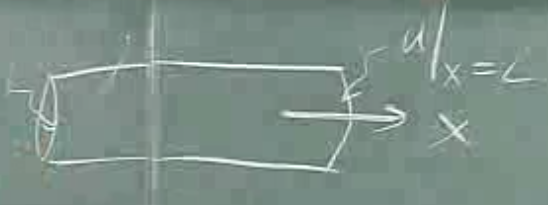
\includegraphics[height=2cm]{1_8.png}

Bu denklem ustteki gibi bir borudaki isinin dagilimini, akisini gosteriyor
olsun. $u|_{x=L}$ ile gosterilen bir sinir sarti, yani $L$ uzunlugundaki
borunun en ucunda (sagindaki) olmasi sart olan isi seviyesi. Mesela bu sart
$u|_{x=L} = T_2$ olsun, ki $T_2$ bir tekil sayi, $100^o$ , $200^o$ gibi. Simdi homojenlige
ne oldu? Ana denklem homojen, ama homojenlik testini sinir sartina uyguladigimiz
zaman $0 = T_2$ gibi bir sonuc aliyoruz, ki bu absurt bir sonuc demek ki sinir
sarti homojen degil. O zaman bu problemin tamami homojen olamaz. 

Benzer sekilde borunun oteki ucu icin tanimlanan sart gayri lineer olsa

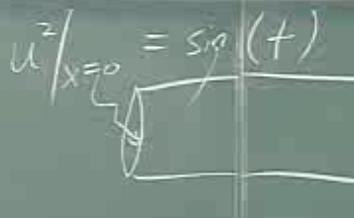
\includegraphics[height=2cm]{1_9.png}

ki bu sart o uctan bir tur sinusoidal bir enerji, isi verildigi bir durumu
tarif ediyor, o zaman ana denklem lineer olsa bile, sinir sartinda gayri
lineerlik oldugu icin problemin tamami gayri lineer olacaktir. 

Aslinda formel olarak sinir sartlarini alip 

\[ \mathcal{L}  = \frac{\partial }{\partial t} - k \partial_{xx}\]

operator tanimina bir sekilde dahil etmenin yollari var, ama biz bunlar cok
ileri seviye teknikler, bu derste bu teknikleri gormeyecegiz. 

Baslangic Sartlari

Mesela yayilma (diffusion) denklemi $u(x,t)$ icin $u(x,0) = f(x)$, yani
baslangic aninda isi dagiliminin tum boru boyunca hangi seviyelerde
oldugunun (burada bu dagilim $f(x)$) belirtilmesi , baslangic sartini
tanimlamak demektir.

Genel bir kural PDE'deki turev sayisi kadar sart tanimlanmasi
gerektigidir. Mesela iki zaman turevi var ise, iki tane kosul gerekir,
mesela $t=0$ anindaki bir kosul, arti zamana goreve turevin $t=0$ anindaki
degeri, vs. 

Soyle dusunebiliriz, $u_{xx}$'in oldugu bir denklemde $u$ elde etmek icin
iki kere entegre edilir, ve bunun sonucu olarak iki tane entegrasyon sabiti
ortaya cikar, ki bu degerler herhangi bir sayi olabilir. O iki sabiti
hesaplamak icin iki tane kosul gerekecektir. 

Genel kurali daha somutlastirirsak, ``her bagimsiz degisken icin gereken
sinir kosulu, o bagimsiz degiskenin derecesine esittir''. Tabii bu genel
bir kural, bazen gercek dunyadaki fizik problemlerinde bu gecerli
olmayabiliyor, bir problem icin duzgun sinir kosullari bulmak basli basina
bir sanat denebilir aslinda. 

Ornek

Laplace denklemi

\[ \nabla^2 u \equiv \frac{\partial ^2u}{\partial x^2} + 
\frac{\partial ^2u}{\partial y^2}  +
\frac{\partial ^2u}{\partial z^2} 
\]

ki $\nabla^2$ Laplacian operatoru olarak bilinir. 

Ustteki turden bir denklem hic kaynak akim verilmeyen sonsuz uzayda
elektrik potansiyeli alanini temsil ediyor olabilir. 

Bu denklemin bir cozumun (ki sinir sartlarina dikkat edelim) su sekilde
oldugunu gostermek kolaydir:

\[ u(\vec{x}) = \frac{1}{\sqrt{x^2+y^2+z^2}} \]

Bu Potansiyel Teori'sinde tipik bir problem, bir alan degiskeni var, ve
orijinden uzaklastikca bu degisken azaliyor, bu azalma $1 / $ uzakligin
karesi oraninda. 

Bu ``bir'' cozum, fakat bir suru 2. derece turev var ortalikta, o zaman
$x,y,z$'nin her turlu lineer fonksiyonu de aslinda bir cozumdur. Mesela

\[ u(\vec{x}) = \alpha x + \beta y + \gamma z + \delta \]

formulu de bir cozum olabilir. Niye? Herhangi bir lineer fonksiyonun iki
kere turevini alirsak o fonksiyon yokolur. 

Demek ki bu problemin tanimi eksik, sinir sartlari da tanimlanmasi gerekli,
aksi takdirde elde edilen sonuclar ozgun olmayacak. Envai turden cozum
mumkun. 

Bu problem icin tipik bir sinir kosulu $\lim_{|\vec{x}|\to \infty} u = 0$
ifadesidir. Elektrik alan ornegine donersek, elektrik alani sonsuzluga
giderken sifira dusuyor demis oluyoruz. Bir sabite gidiyor da diyebilirdik,
o da islerdi. 

O tur bir sart 

\[ u(\vec{x}) = \frac{1}{\sqrt{x^2+y^2+z^2}} \]

sonucunu saglardi, diger secenekleri elemis olurdu. Bu ornegi sinir
kosullarinin onemini belirtmek icin sectik, bu kosullar ana denklemin
kendisi kadar onemli. 

Bir nokta daha:

Soyle bir ODE dusunelim

\[ \frac{du}{dt} = 1 \]

Entegre edince genel cozum

\[ u(t) = t + c_1 \]

Fakat PDE icin

\[ u = u(x,y) \]

\[ u_x = xy \]

Burada $y$ bazli bir turev yok, basit bir PDE, cozmesi kolay, fakat
unutmayin, entegre edince

\[ u = \frac{1}{2}x^2y + [..] \]

Noktalarin oldugu yere ne gelecek? Bir sayi sabiti degil bir fonksiyon
gelecek. 

\[ u = \frac{1}{2}x^2y + g(y) \]

cunku $u$, $y$'nin bir fonksiyonu, o zaman elimize gecen $y$'nin herhangi
bir fonksiyonu olacak, ki bu fonksiyonun degeri sinir kosullari uzerinden
tanimlanmis olmali. Bunu ozellikle vurgulamak istedim cunku insanlar bu
detayi unutabiliyor.

Sinir kosulu nasil olabilir? Mesela $u(\alpha,y) = f(y)$ seklinde
olabilir. Bu kosulu yerine sokunca

\[ \frac{1}{2}\alpha^2 y + g(y) = f(y) \]

Bu bize $g(y)$'in ne oldugunu soyler

\[ g(y)  = f(y) - \frac{1}{2}\alpha^2 y \]

ve bu ornek icin nihai cozum

\[ u(x,y) = \frac{1}{2}x^2y + f - \frac{1}{2}\alpha^2 y \]

Tekrarlamak gerekirse

Bir Kismi Turevsel Denklem (PDE) cok degiskenli bilinmeyen bir fonksiyon ve
o fonksiyonun kismi turevleri arasinda kurulan bir iliskidir. 

Ornek 

\[ u = u(x,t) \]

olmak uzere

\[ \frac{\partial u}{\partial x} + \frac{\partial u}{\partial t} = 0\]

denklemi bir PDE'dir. Cozum bir tek sayisal sonuc degil, bir
fonksiyondur. Dusunelim, mesela $f$ fonksiyonu tek degiskenli ve turevi
alinabilir bir fonksiyon ise

\[ u(x,t) = f(x-t) \]

cozumdur diyebilir miyiz? Yani cozum $f(x-t)$ olabilir mi? Kontrol edelim 

\[ u_x = f'(x-t) \]

\[ u_t = -f'(x-t) \]

Bu iki kismi turev toplaninca sifir cikar, yani sonuc ustte tanimli PDE'ye
uyar. Bu genel tanima uyan bir suru fonksiyon vardir, mesela 

\[ u(x,t) = (x-t)^2 \]

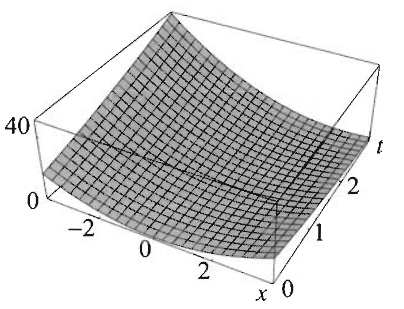
\includegraphics[height=4cm]{1_1.png}

\[ u(x,t) = e^{-(x-t)^2} \]

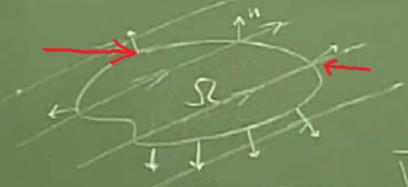
\includegraphics[height=4cm]{1_2.png}

\[ u(x,t) = 3sin(x-t) \]

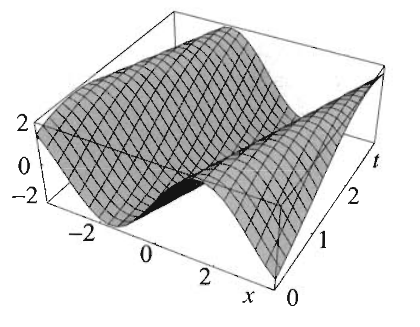
\includegraphics[height=4cm]{1_4.png}

Not: Burada $f$'i bir $f(z)$ olarak gorebiliriz, bu fonksiyona $(x-y)$
geciliyor, yani bir icice fonksiyon ortaya cikiyor. O zaman ustteki formlar
aslinda $f(z) = z^2$, ve $e^{-z^2}$ seklinde. Tabii kismi turevler ile
turev alinca Zincirleme Kanunu devreye girmelidir ve gecilen degerlerin,
``fonksiyonlarin'' da turevi alinmalidir, vs. 

Yani ustteki sonuc aslinda diyor ki $x-t$ seklinde hep beraber olmak uzere
bu ikiliyi kullanan herhangi bir fonksiyon, ustteki PDE'nin cozumudur. Bu
sekilde cozum birden fazla fonksiyon oluyor, ve bu cozum fonksiyonlarinin
birbirinden ne kadar farkli olabildigi, gostermeye calistigimiz noktalardan
biri.

Ustteki PDE bir tasinim (advection) ornegidir, ve 1. seviye lineer homojen
bir denklemdir. 1. seviye en yuksek turev seviyesinin seviyesine isaret
eder, lineer homojen ise tum cozumlerin lineer bir sekildeki kombinasyonu
yine bir cozumdur anlamina gelir. Ustteki PDE icin ne kadar cesitli
cozumler olabildigini gorduk, onlarin kombinasyonlariyla bu cesitlerin daha
da artacagini dusunebiliriz. kiyasla soyle bir ODE icin

\[  y' - y  = 0\]

icin cozumler

\[ y = Ae^x \]

denklemidir Tek bir cozume indirgemek icin baslangic sarti mesela $y(0) =
2$ 
veririz ve oradan tek cozum $y = 2e^x$ buluruz. 

Ornek PDE'miz icin de, benzer sekilde, tek bir fonksiyonu bulmak icin
baslangic, ya da sinir sartlari koymaliyiz. 

Ornek

Ornek PDE cozumleri arasinda hangisi x ekseni boyunca $u = e^{-x^2}$
sartini tatmin eder? 

$u = e^{-x^2}$ demek, $u(x,0)$ demektir, cunku $t$ yoktur. Cozumlerimizi
teker teker gozden gecirirsek, $u(x,0)$ denklemi $u = e^{-x^2}$ olan
cozum

\[ u(x,t) =  e^{-(x-t)^2} \]

cozumudur. Gorsel olarak durumu canlandirmak gerekirse, $t$'yi bir zaman
degiskeni olarak kabul edelim, ve 

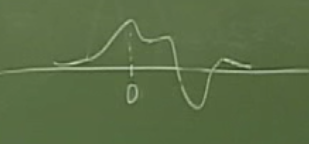
\includegraphics[height=2cm]{1_3.png}

her $t$ degerinde o anda $u$'nun $x$ uzerinde dusen yansimasinin bir
fotografini cekiyoruz sanki, ustteki resimde soldaki $t=0$ anindaki
mesela. 

Devam edelim. Ornek 1 icin bir suru cozumden bahsettik ama bu cozumleri
nasil turettigimizi soylemedik. Ayrica bu ornekte ``tum mumkun cozumleri''
bulup bulmadigimizi da soylemedik. Simdi gosterecegimiz islemler hakikaten
tum cozumleri buldugumuzu gosterecek, ve akillica kullanilabilecek bir
degisken degistirme (change of variables) tekniginin bir problemi
basitlestirmekte nasil faydali olacagini anlatmaya ugrasacak. 

Ornek

Ustteki PDE'yi lineer degisken degisimi kullanarak bir ODE'ye indirgemeye
ugrasacagiz. Diyelim ki

\[ \alpha = a x + b t \]

\[ \beta = cx + dt \]

Kismi turevler $u_x$ ve $u_t$ su sekilde genisletilebilir

\[ u_x = 
\frac{\partial u}{\partial \alpha}\frac{\partial \alpha}{\partial x}  +
\frac{\partial u}{\partial \beta}\frac{\partial \beta}{\partial x} 
\]


\[ u_t = 
\frac{\partial u}{\partial \alpha}\frac{\partial \alpha}{\partial t}  +
\frac{\partial u}{\partial \beta}\frac{\partial \beta}{\partial t} 
\]

Ilk bastaki degisken degisimine gore bazi kismi turevler soyle:

\[ \frac{\partial \alpha}{\partial x} = a , \ \frac{\partial \alpha}{\partial t} = b, \ \frac{\partial \beta}{\partial x} = c , \
\frac{\partial \beta}{\partial t} = d 
\]

Bunlari $u_x$ ve $u_t$ icinde yerlerine gecirirsek,

\[ u_x = 
\frac{\partial u}{\partial \alpha} a +
\frac{\partial u}{\partial \beta} c
\ \ \ (1)
\]

\[ u_t = 
\frac{\partial u}{\partial \alpha} b +
\frac{\partial u}{\partial \beta} d
\ \ \ (2)
\]

Ustteki iki kismi turevi ana PDE'de yerine koyarsak

\[ \frac{\partial u}{\partial x} + \frac{\partial u}{\partial t} = 0\]

soyle olur

\[ 
\frac{\partial u}{\partial \alpha} a  +
\frac{\partial u}{\partial \beta} c + 
\frac{\partial u}{\partial \alpha} b + 
\frac{\partial u}{\partial \beta} d = 0
\]

Benzer terimleri gruplayalim

\[ 
\frac{\partial u}{\partial \alpha} (a+b)
\frac{\partial u}{\partial \beta} (c+d) = 0
\]

Simdi oyle $a,b,c,d$ degerleri secelim ki bir kismi turev yokolsun. Mesela 

\[ a = 1, b = 0, c=1, d=-1 \]


O zaman 

\[ \frac{\partial u}{\partial \alpha} = 0 \]

kalir. Bu artik bir basit diferansiyel denklemdir, cozum icin entegral
aliriz, 

\[ u = C(\beta) \]

Unutmayalim, sifirin entegrali bir sabittir, ama $u$ birden fazla degiskene
sahip oldugu icin bu ``sabitin'' $\beta$ icermesi gerekir. $C(\beta)$,
$\alpha$'ya gore bir sabittir. 

$C(\beta)$'yi daha somutlastiralim, 

\[ \beta = cx + dt \]
 
demistik, ayrica $c=1,d=-1$. O zaman cozum

\[ u = C(x-t) \]

Bu da basta buldugumuz cozum ile ayni zaten. 






\end{document}
